%class
	\documentclass{beamer}

%template
	\usetheme{HannoverSalman}
	\setbeamertemplate{navigation symbols}{}
	%\setbeamertemplate{footline}{\centering{\insertframenumber/\insertpresentationendpage}}
	%\setbeamertemplate{footline}{\hspace*{.5cm}\scriptsize{\hfill\insertframenumber\hspace*{.5cm}}} 


%packages
	\usepackage{amsmath, amssymb, graphicx,cancel}
	\usepackage[absolute,overlay]{textpos}
	\usepackage{subfigure}
	\usepackage{caption}\captionsetup{labelformat=empty,labelsep=none}
	\usepackage{geometry}
	\geometry{verbose}
	\usepackage{color}
	\usepackage{xmpmulti}
	\usepackage[3D]{movie15}
	\usepackage{hyperref}
%	\usepackage{bookmark}
	\usepackage[open,openlevel=4,atend]{bookmark}
	%\bookmarksetup{color=blue}
	\usepackage{multirow}
	\usepackage[style=numeric,defernumbers, authoryear]{biblatex}
	%\usepackage[square,sort]{natbib}
	%\usepackage{fancyhdr}%\pagestyle{fancy} 

	
	\hypersetup{bookmarksdepth = 4}


%citations files
	\bibliography{MyCitations}

%logoCSIPCPL
    \setlength{\TPHorizModule}{1mm}
    \setlength{\TPVertModule}{1mm}
    \newcommand{\logoCSIPCPL}
    {
    	\begin{textblock}{1}(100,2) %(100,85)  for bottom
    		
\includegraphics[width=1.5cm]{figs/logo_CSIP}
    	\end{textblock}
    	
	\begin{textblock}{1}(117,1) %(117,85)  for bottom
    		
\includegraphics[width=1.0cm]{figs/logo_CPL}
    	\end{textblock} 
    }

%logo evolution
    \newcommand{\logoEvolution}
    {    	
	\begin{textblock}{1}(110,1) %(117,85)  for bottom
    		\includegraphics[width=0.65in]{figs/logo_evolution.pdf}
    	\end{textblock} 
    }

%logo Qualcomm
    \newcommand{\logoQualcomm}
    {
    	\begin{textblock}{1}(110,2) %(100,85)  for bottom
    		\includegraphics[width=1.5cm]{figs/logo_qualcomm.jpg}
    	\end{textblock}
    }
%logo Qualcomm (long)
    \newcommand{\logoQualcommllong}
    {
    	\begin{textblock}{1}(0,0) 
    		\includegraphics[width=1.25in]{figs/logo_qualcomm_long.jpg}
    	\end{textblock}
    }

%logo Tech Tower
    \newcommand{\logoTechTower}
    {
    	\begin{textblock}{1}(0,0) 
    		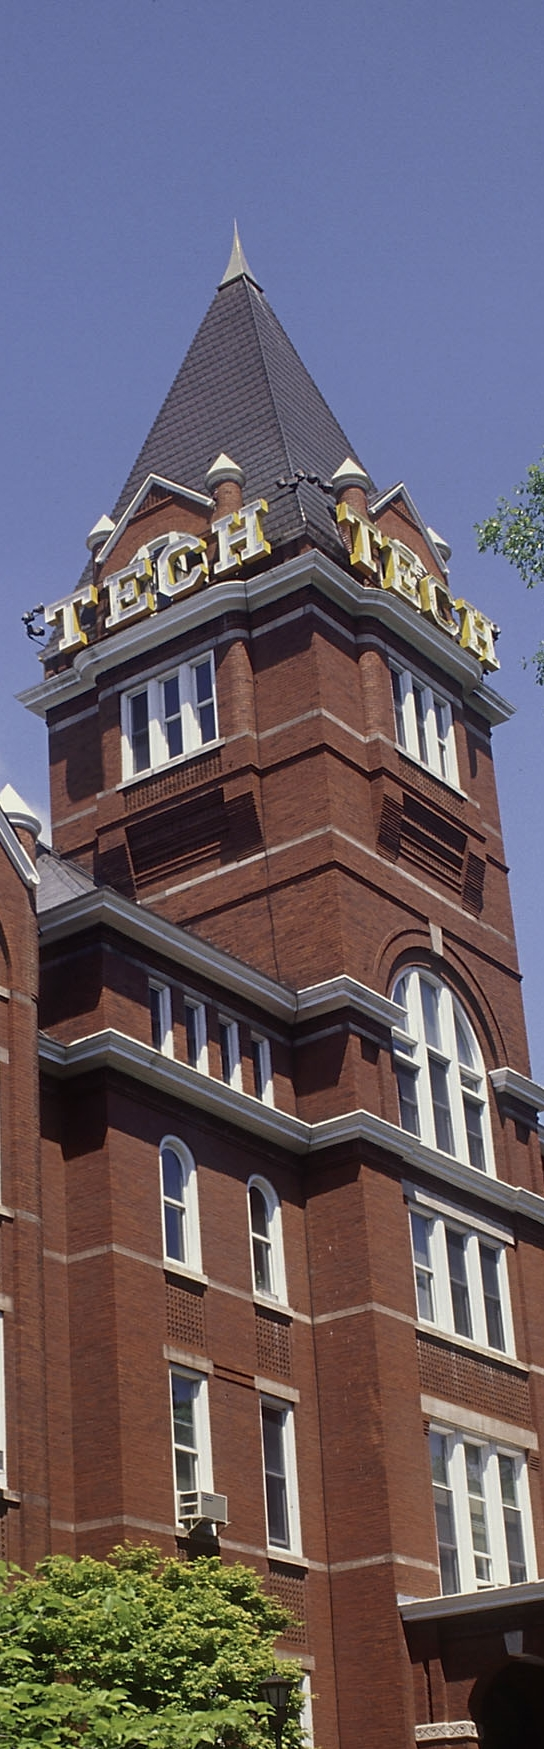
\includegraphics[width=1.25in]{figs/logo_TechTower.jpg}
    	\end{textblock}
    }

%logo tree
    \newcommand{\logoTree}
    {
    	\begin{textblock}{1}(0,0) 
    		\includegraphics[width=1.25in]{figs/logo_tree.jpg}
    	\end{textblock}
    }
%page numbers
    \newcommand{\mypagenum}
    {
    	\begin{textblock}{1}(1,94) 
		{\tiny \color[rgb]{0.2,0.2,1}\insertframenumber} %\insertframenumber,\insertpresentationendpage, \inserttotalframenumber
    	\end{textblock}
    }
%my footnote citation
	\newcommand{\myFootnoteCitation}[2]
	{
		\footnote{\tiny \citeauthor{#1}, \emph{#2}, \citeyear{#1}.}  %\citeauthor{#1}, \citetitle{#1}, #2 \citeyear{#1}.
	}
%my refer to citation
	\newcommand{\mycite}[1]
	{
		\emph{\citeauthor{#1} (\citeyear{#1})}
	}
%my footnote website citation
	\newcommand{\myFootnoteWebsiteCitation}[1]
	{
		\footnote{\tiny \citeauthor{#1}}
	}

\let\thefootnote\relax\footnotetext{Footnotetext without footnote mark}


%section underline
%\newcommand{\tmpsection}[1]{}
%\let\tmpsection=\section
%\renewcommand{\section}[1]{\tmpsection{\underline{#1}}}



%commands
	\newcommand{\likelihood}{p(Z_k| x_k) }						%likelihood
	\newcommand{\prior}{p(x_k)  } 								%prior
	\newcommand{\posterior} {p(x_k| Z_k)}						%posterior
	\newcommand{\prediction} {p(x_k| Z_{k-1})}					%prediction
	\newcommand{\update} {p(x_k|Z_k)}							%update
	\newcommand{\observations} {p(Z_k)}						%observations
	\newcommand{\prevobservations} {p(Z_{k-1})}				%previous observations
	\newcommand{\dxpk} {dx_{k-1}}							%dx_{k-1}
	\newcommand{\ChapKolm}{\int{p(x_k| x_{k-1})p(x_{k-1}|Z_{k-1})} \dxpk} %Chapman Kolmogorov

	%algorithm specific: JPDAF
	\newcommand{\likelihoodJPDAF}{p(Z_k| \chi, m, Z_{k-1}) }		%1. likelihood
	\newcommand{\priorJPDAF}{p(\chi|m, Z^{k-1}} 				%2. prior	
	\newcommand{\observationsJPDAF} {p(Z_k}					%3. observations
	\newcommand{\posteriorJPDAF} {p(\chi| Z_k)}					%4. posterior

%environments
	\newenvironment{changemargin}[2]
	{
	  	\begin{list}{}
		{
			\setlength{\topsep}{0pt}%
			\setlength{\leftmargin}{#1}%
			\setlength{\rightmargin}{#2}%
			\setlength{\listparindent}{\parindent}%
			\setlength{\itemindent}{\parindent}%
			\setlength{\parsep}{\parskip}%
		}
	  	\item[]
		}
		{\end{list}
	}
%figures

%colors
\definecolor{darkgreen}{rgb}{0,0.5,0}

%personal details
	\author{Salman Aslam}
	\institute{Advisor, Dr Christopher Barnes (ECE)\\Co-advisor, Dr Aaron Bobick (CoC)\\Georgia Institute of Technology}
	\date{}

\begin{document}
%####################################################################################################
\title{Image Processing}
%####################################################################################################
\begin{frame}[plain]\logoTechTower
	\titlepage
\end{frame}

\begin{frame}
\frametitle{Outline}
\logoCSIPCPL\logoTechTower
	\setcounter{tocdepth}{1}	
	\tableofcontents
\end{frame}


%#######################################################################
\section{INTRODUCTION}
%####################################################################################################

%#######################################################################
\section{SEGMENTATION}
%####################################################################################################

\begin{frame}
\frametitle{Overview}
\logoCSIPCPL\mypagenum
	Processing images can be distinguished into two levels:

	\begin{enumerate}
		\item \emph{Low level processing}.  Low level processing often includes image restoration, noise filtering and image compression.  In essence, it is about increasing image quality for better viewer perception or decreasing image size for efficient transmission and storage.  
		\item \emph{High level processing}.   High level processing includes extracting features or objects of interest from the image and trying to understand, recognize or classify them. The essence here is understanding image content.
	\end{enumerate}
\end{frame}



\begin{frame}
\frametitle{Overview}
\logoCSIPCPL\mypagenum
	\begin{figure}[!htp]
		\includegraphics[width=2in]{figs/segmentation_YoungWomanOldLady.jpg}
		\caption{\emph{My wife and my mother-in-law}, published in 1915 by the cartoonist W.E. Hill.  The chin of the young woman becomes the nose of the old lady. } 
		\label{fig:YoungWomanOldLady}
	\end{figure}
\end{frame}





\begin{frame}
\frametitle{Overview}
\logoCSIPCPL\mypagenum
	\begin{itemize}
		\item Image segmentation can be considered to be the bridge between low and high level processing.
		\item At one end, it shares some techniques with low level processing, the most notable of which is edge detection.
		\item On the other end, image segmentation is normally the first step in a high level processing system.
	\end{itemize}
\end{frame}





\begin{frame}
\frametitle{Overview}
\logoCSIPCPL\mypagenum
	\begin{block}{Definition:}
		The goal of Segmentation is to take an input image and clearly separate the objects in it.
	\end{block}
	\begin{block}{Mathematically:}
		Segmentation of an image $f$ is a finite set of regions $f_1, f_2 ... f_N$ such that
		\begin{equation}
			f=\bigcup_{i=1}^{i=N} f_i \ \ \ \ \ \ \ \ \ f_i \cap f_j = \phi
		\end{equation}
	\end{block}
\end{frame}







%===================================================
\subsection{\ \ \ \ 1. Thresholding}
%===================================================
\begin{frame}
\frametitle{Thresholding based methods}
\logoCSIPCPL\mypagenum
	\begin{block}{Definition:}  
		A family of segmentation methods in which the histogram is used to find one or several thresholds that will effectively partition the image into different foreground objects and background.
	\end{block}
\end{frame}



\begin{frame}\frametitle{Thresholding based methods}
\logoCSIPCPL\mypagenum
	Types of thresholding:
	\begin{itemize}
		\item Global thresholding
		\begin{itemize}
			\item Binary thresholding
			\item Multilevel thresholding
		\end{itemize}
		\item Local thresholding
	\end{itemize}
	
	Global thresholds can be computed automatically using:
	\begin{itemize}
		\item Automatic thresholding
		\begin{itemize}
			\item Automatic binary thresholding
			\item Automatic multilevel thresholding (K-means clustering)
		\end{itemize}
		\item Optimal thresholding
	\end{itemize}
\end{frame}





\begin{frame}
\frametitle{Thresholding based methods}
\logoCSIPCPL\mypagenum
	Since thresholding depends on histograms, it would be worthwhile to discuss different kinds of histograms:
	\begin{itemize}
		\item Unimodal: One mode (trivial case)
		\item Bimodal: Two modes separated by a clear valley
		\item Multimodal: Multiple modes separated by clear valleys
		\item Non-modal: No modes at all, or no clear valleys between modes
	\end{itemize}
\end{frame}





\begin{frame}
\frametitle{Thresholding based methods}
\logoCSIPCPL\mypagenum
	\begin{figure}[!htp]
		\includegraphics[width=2in]{figs/segmentation_HistogramMultimodal.jpg}
		\caption{Multimodal histogram}
	\end{figure}
\end{frame}





\begin{frame}
\frametitle{Thresholding based methods}
\framesubtitle{Binary thresholding}
\logoCSIPCPL\mypagenum
	\begin{block}{Definition:}Thresholding method in which one threshold is used to separate foreground objects from the background.
	\end{block}
	\begin{block}{Mathematically:}
		\begin{equation}
			g(m,n) = 
			\begin{cases}
				0 & \text{if $f[m,n] < T$} \\
				1 & \text{if $f[m,n] \geq T$}
			\end{cases}
		\end{equation}
	\end{block}
\end{frame}




\begin{frame}
\frametitle{Binary thresholding}
\logoCSIPCPL\mypagenum
	Binary thresholding can only be used under the following conditions:
	\begin{itemize}
		\item All pixels for all foreground objects are either greater or less in value than the background pixels.  This will ensure that no foreground object is merged into the background.
		\item Foreground objects do not overlap.  All foreground objects will be given the same pixel value, but nevertheless will appear distinct from each other.
	\end{itemize}
\end{frame}




\begin{frame}
\frametitle{Multilevel thresholding}
\logoCSIPCPL\mypagenum
	\begin{block}{Definition:}
		Thresholding method in which several thresholds are used to separate foreground objects from the background.
	\end{block}

	\begin{block}{Mathematically:}
		\begin{equation}
			g(m,n) = 
			\begin{cases}
				0 & \text{if  \ \ \ \ \ \ \ \ \ \  \ $f[m,n] < T_1$} \\
				1 & \text{if  \ $T_1 \ \ \ \leq  f[m,n] < T_2 $} \\
				2 & \text{if  \ $T_2 \ \ \ \leq  f[m,n] < T_3 $} \\
				3 & \text{if  \ $T_3 \ \ \ \leq  f[m,n] < T_4 $} \\
				... \\
				N & \text{if \  $T_{N} \ \ \ \leq  f[m,n]$} \\
			\end{cases}
		\end{equation}
	\end{block}
\end{frame}







\begin{frame}
\frametitle{Multilevel thresholding}
\logoCSIPCPL\mypagenum
Multilevel thresholding can only be used under the following
conditions:
	\begin{itemize}
	\item All pixels for all foreground objects are distinct from background pixels.
	\item Foreground objects either do not overlap, and if they do overlap, they have distinct pixel values.
	\end{itemize}
\end{frame}




\begin{frame}
\frametitle{Effect of illumination}
\logoCSIPCPL\mypagenum
	\begin{itemize}
		\item So far, we have shown how to segment a bimodal or multimodal histogram (under certain conditions)
		\item Unfortunately, a non-modal histogram cannot be segmented effectively using thresholding
		\item However, in some cases, it may be possible to transform a non-modal histogram into a binary or multilevel histogram
		\item An example of when this may be possible is if the image was captured under non-uniform illumination.
	\end{itemize}
\end{frame}







\begin{frame}
\frametitle{Effect of illumination}
\logoCSIPCPL\mypagenum
	\begin{itemize}
		\item Simple model of image generation is that an image $f[m,n]$ is the product of a reflectance component $r(m,n)$ and an illumination component $i(m,n)$,
			\begin{equation}\label{Eqn:OriginalImageGeneration}
				f[m,n] = r[m,n] * i[m,n]
			\end{equation}
		\item If $r[m,n]$ has a bimodal histogram but $i[m,n]$ is non-uniform, $f[m,n]$ could end up with a non-modal histogram
		\item The histogram can be made bimodal again if access to the illumination source is available
	\end{itemize}
\end{frame}






\begin{frame}
\frametitle{Local thresholding}
\logoCSIPCPL\mypagenum
	\begin{block}{Definition:} 
		Local thresholding is a special case of global thresholding.  It is global thresholding applied to different parts of an image.
	\end{block}
\end{frame}





\begin{frame}
\frametitle{Automatic binary thresholding}
\logoCSIPCPL\mypagenum
	\begin{block}{Definition:}
		Binary thresholding in which the threshold is automatically selected.
	\end{block}
\end{frame}





\begin{frame}\frametitle{Automatic binary thresholding}\logoCSIPCPL\mypagenum
	The procedure for automatic binary thresholding is:
	\begin{itemize}
		\item \textbf{Select an arbitrary threshold.}  Select an initial global threshold, $T$. A good starting point would be the mean of the minimum and maximum gray level values in the image.
		\item \textbf{Create 2 clusters (i.e. segment image).}  Segment the image using threshold $T$. The group of all intensity values in the image that fall below the threshold are called $C_1$, i.e. the first cluster. Similarly, the group of all intensity values in the image that fall above the threshold are called $C_2$, i.e. the second cluster.
	\end{itemize}
\end{frame}


\begin{frame}
\frametitle{Automatic binary thresholding}
\logoCSIPCPL\mypagenum
	\begin{itemize}
		\item \textbf{Compute centroids.}  Compute centroids $\mu_1$ and $\mu_2$.  These are the means of $C_1$ and $C_2$ respectively.
		\item \textbf{Update threshold.}  The new threshold $T$ is the mean of $\mu_1$ and $\mu_2$.
		\item \textbf{Repeat till convergence.}  Repeat steps 2 to 4 until successive values of the threshold $T$ are the same.
	\end{itemize}
\end{frame}







\begin{frame}
\frametitle{Thresholding based methods} 
\framesubtitle{Automatic multilevel thresholding (K-means clustering)}
	\begin{block}{Definition:}
		Multilevel thresholding in which the threshold is automatically selected.
	\end{block}
\end{frame}





\begin{frame}
\frametitle{Automatic multilevel thresholding (K-means Clustering)}
\logoCSIPCPL\mypagenum
	The procedure for automatic multilevel thresholding is:
	\begin{itemize}
		\item \textbf{Select $K$ centroids.}  Select an initial $K$ number of centroids, $\mu_1, \mu_2, ... \mu_k$.  A good starting point would be equally spaced intensity values between the minimum and maximum intensity values in the image.
		\item \textbf{Create $K$ clusters (i.e. segment image).}  Segment the image using centroids $\mu_1, \mu_2, ... \mu_k$. This is done by scanning the image, and for every pixel, finding the distance between it and all the centroids.  Then whichever centroid is closest, this pixel is assigned to that centroid.  As more and more pixels are assigned to the centroids, $K$, clusters $C_1, C_2, \ldots C_k$ are formed around the $K$ centroids.\\
	\end{itemize}
\end{frame}








\begin{frame}
\frametitle{Automatic multilevel thresholding (K-means  Clustering)}
\logoCSIPCPL\mypagenum
	\begin{itemize}
		\item \textbf{Update centroids.}  For each cluster, find its updated centroid.
		\item \textbf{Repeat till convergence.}  Repeat steps 2 to 3 until successive values of the centroids are the same.
	\end{itemize}
\end{frame}






\begin{frame}
\framesubtitle{Optimal thresholding}
\logoCSIPCPL\mypagenum
	\begin{block}{Definition:}A thresholding method in which probability of misclassification error is minimized.  The error relates to improperly classifying foreground object pixels as background and vice versa.
	\end{block}
\end{frame}





\begin{frame}
\framesubtitle{Optimal thresholding}
\logoCSIPCPL\mypagenum
	\begin{itemize}
		\item Can use this method if we have some prior knowledge about the distributions of the gray level values that make up the foreground objects and background
		\item This method allows us to compute a threshold that minimizes thresholding errors, i.e. errors of misclassifying foreground object pixels as background pixels and vice versa.
	\end{itemize}
\end{frame}






\begin{frame}
\frametitle{Optimal thresholding}
\logoCSIPCPL\mypagenum
	\begin{itemize}
		\item Assume that the background pixels have probability density function $p_1(x)$
		\item Foreground object pixels have probability density function $p_2(x)$.
		\item We arbitrarily choose a threshold $T$. The error of misclassifying foreground object pixels as background pixels is
		\begin{equation}
			\int_{-\infty}^{T} p_2(x) dx
		\end{equation}
	\end{itemize}
\end{frame}







\begin{frame}
\frametitle{Optimal thresholding}
\logoCSIPCPL\mypagenum
	\begin{itemize}
		\item The error of misclassifying background pixels as foreground object pixels is
			\begin{equation}
				\int_{T}^{\infty} p_1(x) dx
			\end{equation}
		\item If the fraction of the pixels that make up the object is $\rho$, then the total error is
			\begin{equation}
				e(t) = \rho\int_{-\infty}^{T} p_2(x) dx + (1-\rho) \int_{t}^{\infty}p_1(x) dx
			\end{equation}
	\end{itemize}
\end{frame}





\begin{frame}
\frametitle{Optimal thresholding}
\logoCSIPCPL\mypagenum
	\begin{itemize}
		\item We would like to choose threshold $T$ so that the error of
		misclassifying object or background pixels $e(t)$ is minimum.
		\item To do this, we take the first derivative of $e(t)$ with respect
		to $t$, and set it to zero.  The result is,
		\begin{align*}
			\frac{\partial{e}}{\partial{T}}&=\rho p_2(T) - (1-\rho) p_1(T) = 0 \Rightarrow \\
			\rho.p_2(T)  &= (1-\rho).p_1(T)
		\end{align*}	
	\end{itemize}
\end{frame}





%===================================================
\subsection{\ \ \ \ 2. Region}
%===================================================

\begin{frame}
\frametitle{Region based methods}
\logoCSIPCPL\mypagenum
	\begin{block}{Definition:}
		A family of segmentation methods that combine thresholding with the constraint that segmented foreground objects should be connected.
	\end{block}
\end{frame}



%----------------------------------------------------------
\subsubsection{\ \ \ \ \ \ \ \ Growing}
%----------------------------------------------------------
\begin{frame}
\frametitle{Region growing}
\logoCSIPCPL\mypagenum
	\begin{block}{Definition:}
		Region growing methods start with an arbitrary set of seed pixels and grow these pixels to form homogeneous connected regions.
	\end{block}
	\begin{block}{Mathematically:}
		A pixel $x$ will be included in a certain region $R_i$ at iteration $t$ if some function $h$ tests the similarity criterion for pixel $x$ and region $R_i$ and returns true,
		\begin{equation}
			h(R_i^{(t)} \cup x) = TRUE \label{eqn:RegionGrowing}
		\end{equation}
	\end{block}
\end{frame}






\begin{frame}
\frametitle{Region growing}
\logoCSIPCPL\mypagenum
	Region growing is done in the following manner:
	\begin{itemize}
		\item \textbf{Select $k$ seed points.}  Select an initial $k$ number of seed points, $s_1, s_2, ... s_k$.  These are the initial $k$ regions comprising one pixel each.\\
		\item \textbf{Grow $k$ homogeneous regions.} For each region $R_i$, check the 8-point neighborhood of each of its border pixels.  Of all the pixels checked, include those pixels in this region that satisfy the similarity criterion in Eq. (\ref{eqn:RegionGrowing}).\\
		\item \textbf{Repeat until stopping condition met.} Repeat step 2 until a stopping condition is met.
	\end{itemize}
\end{frame}







%----------------------------------------------------------
\subsubsection{\ \ \ \ \ \ \ \ Splitting}
%----------------------------------------------------------
\begin{frame}
\frametitle{Region splitting}
\logoCSIPCPL\mypagenum
	\begin{block}{Definition:}
		A region based method in which the image is initially considered homogeneous and is then successively split into different regions.
	\end{block}	
	\begin{block}{Mathematically:}
		A region $R_i$ will be split into four regions at iteration $t$ if some function $h$ tests the homogeneity criterion for $R_i$ and returns false,
		\begin{equation}
			h(R_i^{(t)}) = FALSE \label{eqn:RegionSplitting}
		\end{equation}
	\end{block}
\end{frame}







\begin{frame}
\frametitle{Region splitting}
\logoCSIPCPL\mypagenum
	Region splitting is done in the following manner:	
	\begin{itemize}
		\item \textbf{Start with entire image.}  Start with the entire image and consider it to be one region.
		\item \textbf{Split regions into four.} Test the homogeneity criterion for each region $R_i$ as given in Eq. (\ref{eqn:RegionSplitting}).  Split $R_i$ into four subregions if it fails the homogeneity test.
		\item \textbf{Repeat until no more splitting possible.} Repeat step 2 until splitting is no longer possible.
	\end{itemize}
\end{frame}




\begin{frame}
\frametitle{Region based methods} 
\framesubtitle{Region splitting}
\logoCSIPCPL\mypagenum
\begin{figure}[!htp]
\begin{center}
\subfigure[Input image.]{
    \label{fig:sub:a}
    \includegraphics[width=2in]{figs/segmentation_Mandril_gray_128x128.jpg}}
    \hspace{0.1cm}
\subfigure[Output image.]{
    \label{fig:sub:a}
    \includegraphics[width=2in]{figs/segmentation_RegionSplitting_T75_OutputImage.jpg}}
\end{center}\end{figure}
\end{frame}






%-----------------------------------------------------------
\subsubsection{\ \ \ \ \ \ \ \ Split and merge}
%-----------------------------------------------------------
\begin{frame}
\frametitle{Region split and merge}
\logoCSIPCPL\mypagenum
	\begin{block}{Definition:}
		A region based method in which any adjacent homogeneous regions created by region splitting are merged immediately after the region splitting.
	\end{block}
	\begin{block}{Mathematically:}  
		At iteration $t$, region splitting is carried out as before.  This is followed by region merging such that two regions $R_i$ and $R_j$ will be merged if they satisfy the homogeneity criterion $h$ such that,
		\begin{equation}
			h(R_i^{(t)} \cup R_j^{(t)}) = TRUE \label{eqn:RegionSplittingAndMerging}
		\end{equation}
	\end{block}
\end{frame}








\begin{frame}
\frametitle{Region split and merge}
\logoCSIPCPL\mypagenum
	\begin{itemize}
		\item \textbf{Start with entire image.}  Start with the entire image and consider it to be one region.
		\item \textbf{Split regions into four.}  Test the homogeneity criterion for each region $R_i$ as given in Eq.
		(\ref{eqn:RegionSplitting}). Split $R_i$ into four subregions if it fails the homogeneity test.
		\item \textbf{Merge regions.}  Merge adjacent regions $R_i$ and $R_j$ if they satisfy Eq. (\ref{eqn:RegionSplittingAndMerging}).
		\item \textbf{Repeat until no more splitting or merging possible.} Repeat steps 2 to 3 until splitting or merging is no longer possible.
	\end{itemize}
\end{frame}





%-----------------------------------------------------------
\subsubsection{\ \ \ \ \ \ \ \ Mean shift}
%-----------------------------------------------------------
\begin{frame}
\frametitle{Mean shift {\small(adaptive gradient ascent)}}
\logoCSIPCPL\mypagenum
	\begin{figure}				
		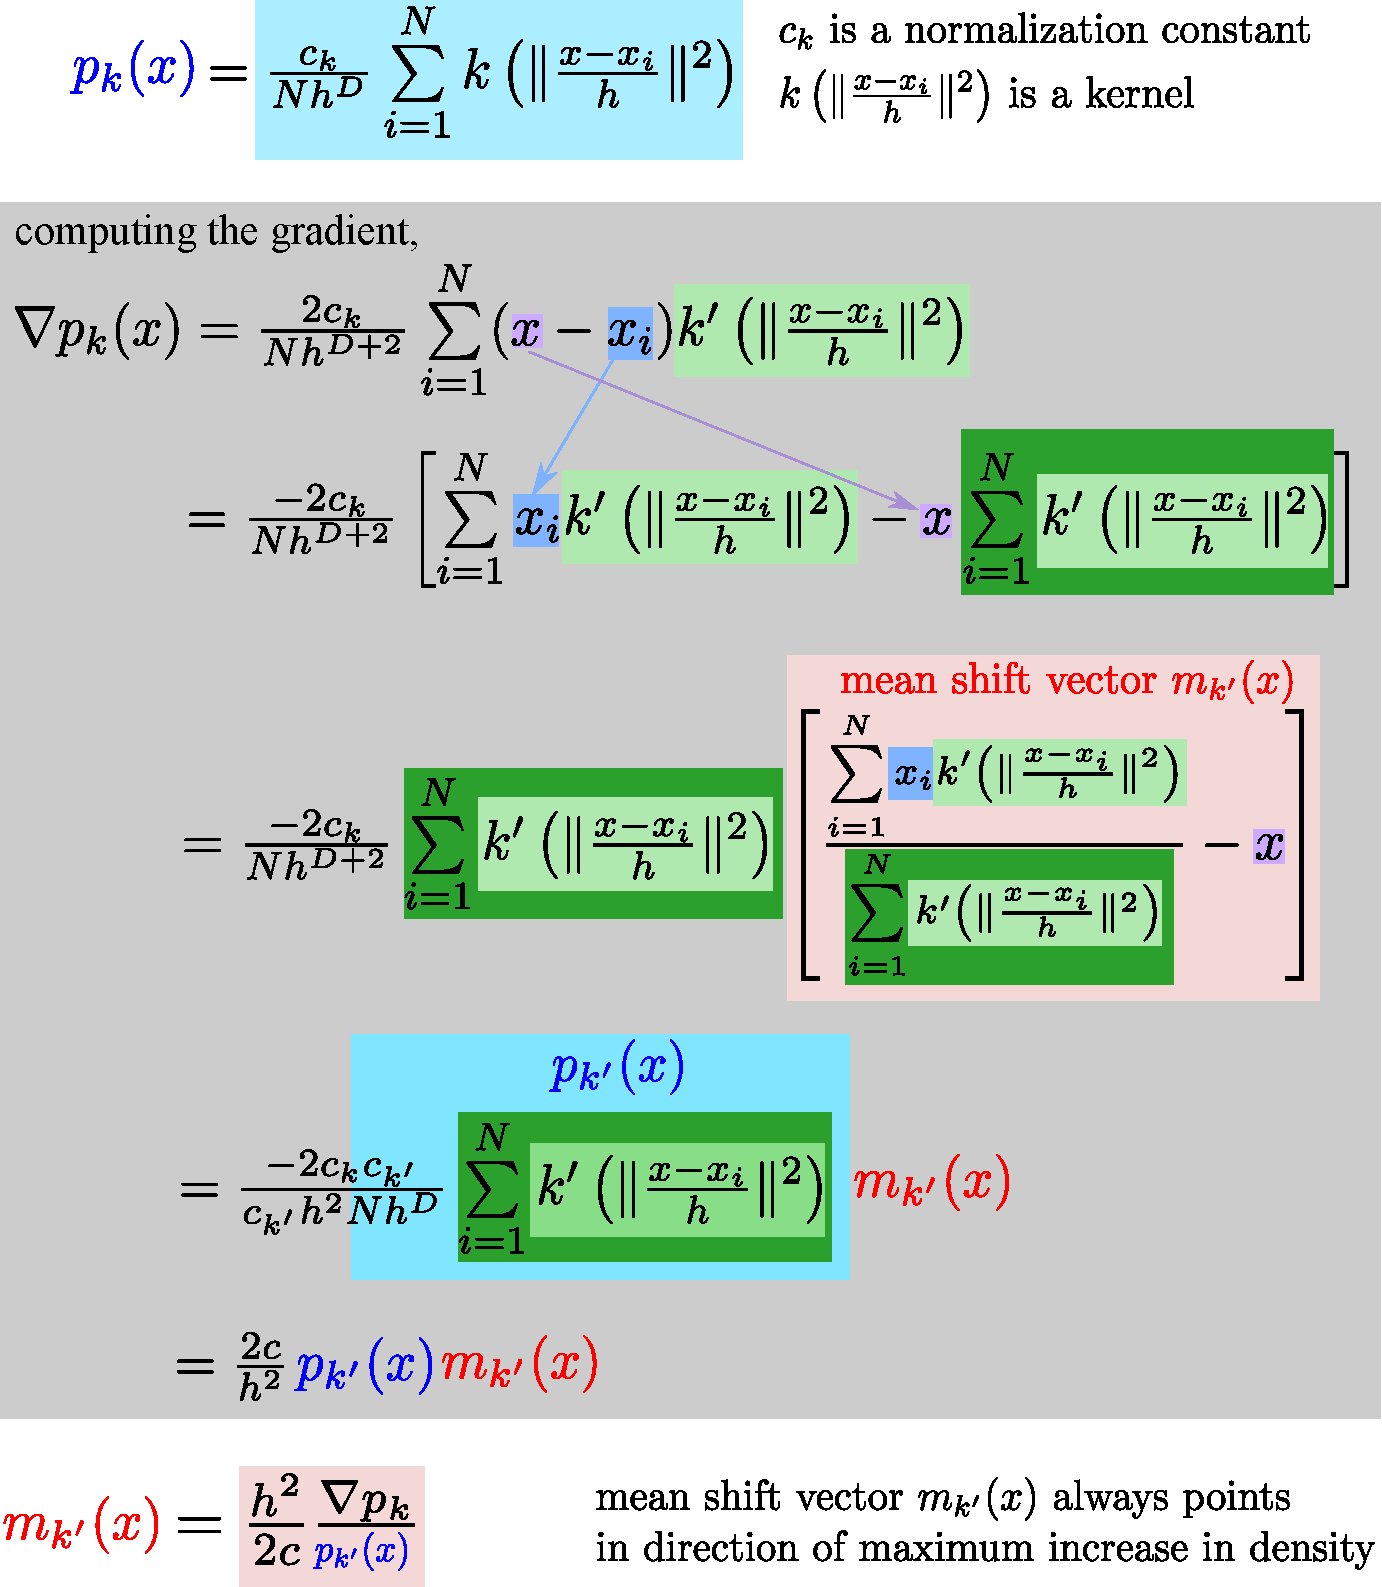
\includegraphics[height=.85\textheight]{figs/PRML_meanShift.pdf}
	\end{figure}
\end{frame}



\begin{frame}\frametitle{Mean shift segmentation}\logoCSIPCPL\mypagenum
	\begin{itemize}				
		\item For a pixel, compute its mean shift vector
		\item This mean shift vector ends at a mode of the density
		\item Repeat for all pixels, now you have a bunch of modes
		\item The set of all locations that converge to the same mode defines the  {\color{red}\emph {basin of attraction}} of that mode
		\item Merge (i.e. prune) modes that are close to each other, and corresponding basins of attraction
	\end{itemize}
\end{frame}




\begin{frame}
\frametitle{Mean shift segmentation\footnote{Comaniciu et. al., 2002}}
\logoCSIPCPL\mypagenum
	\begin{itemize}				
		\item 7 pruned nodes
		\item 7 corresponding basins of attraction (i.e. clusters, or segmented regions)
	\end{itemize}
	\begin{figure}
		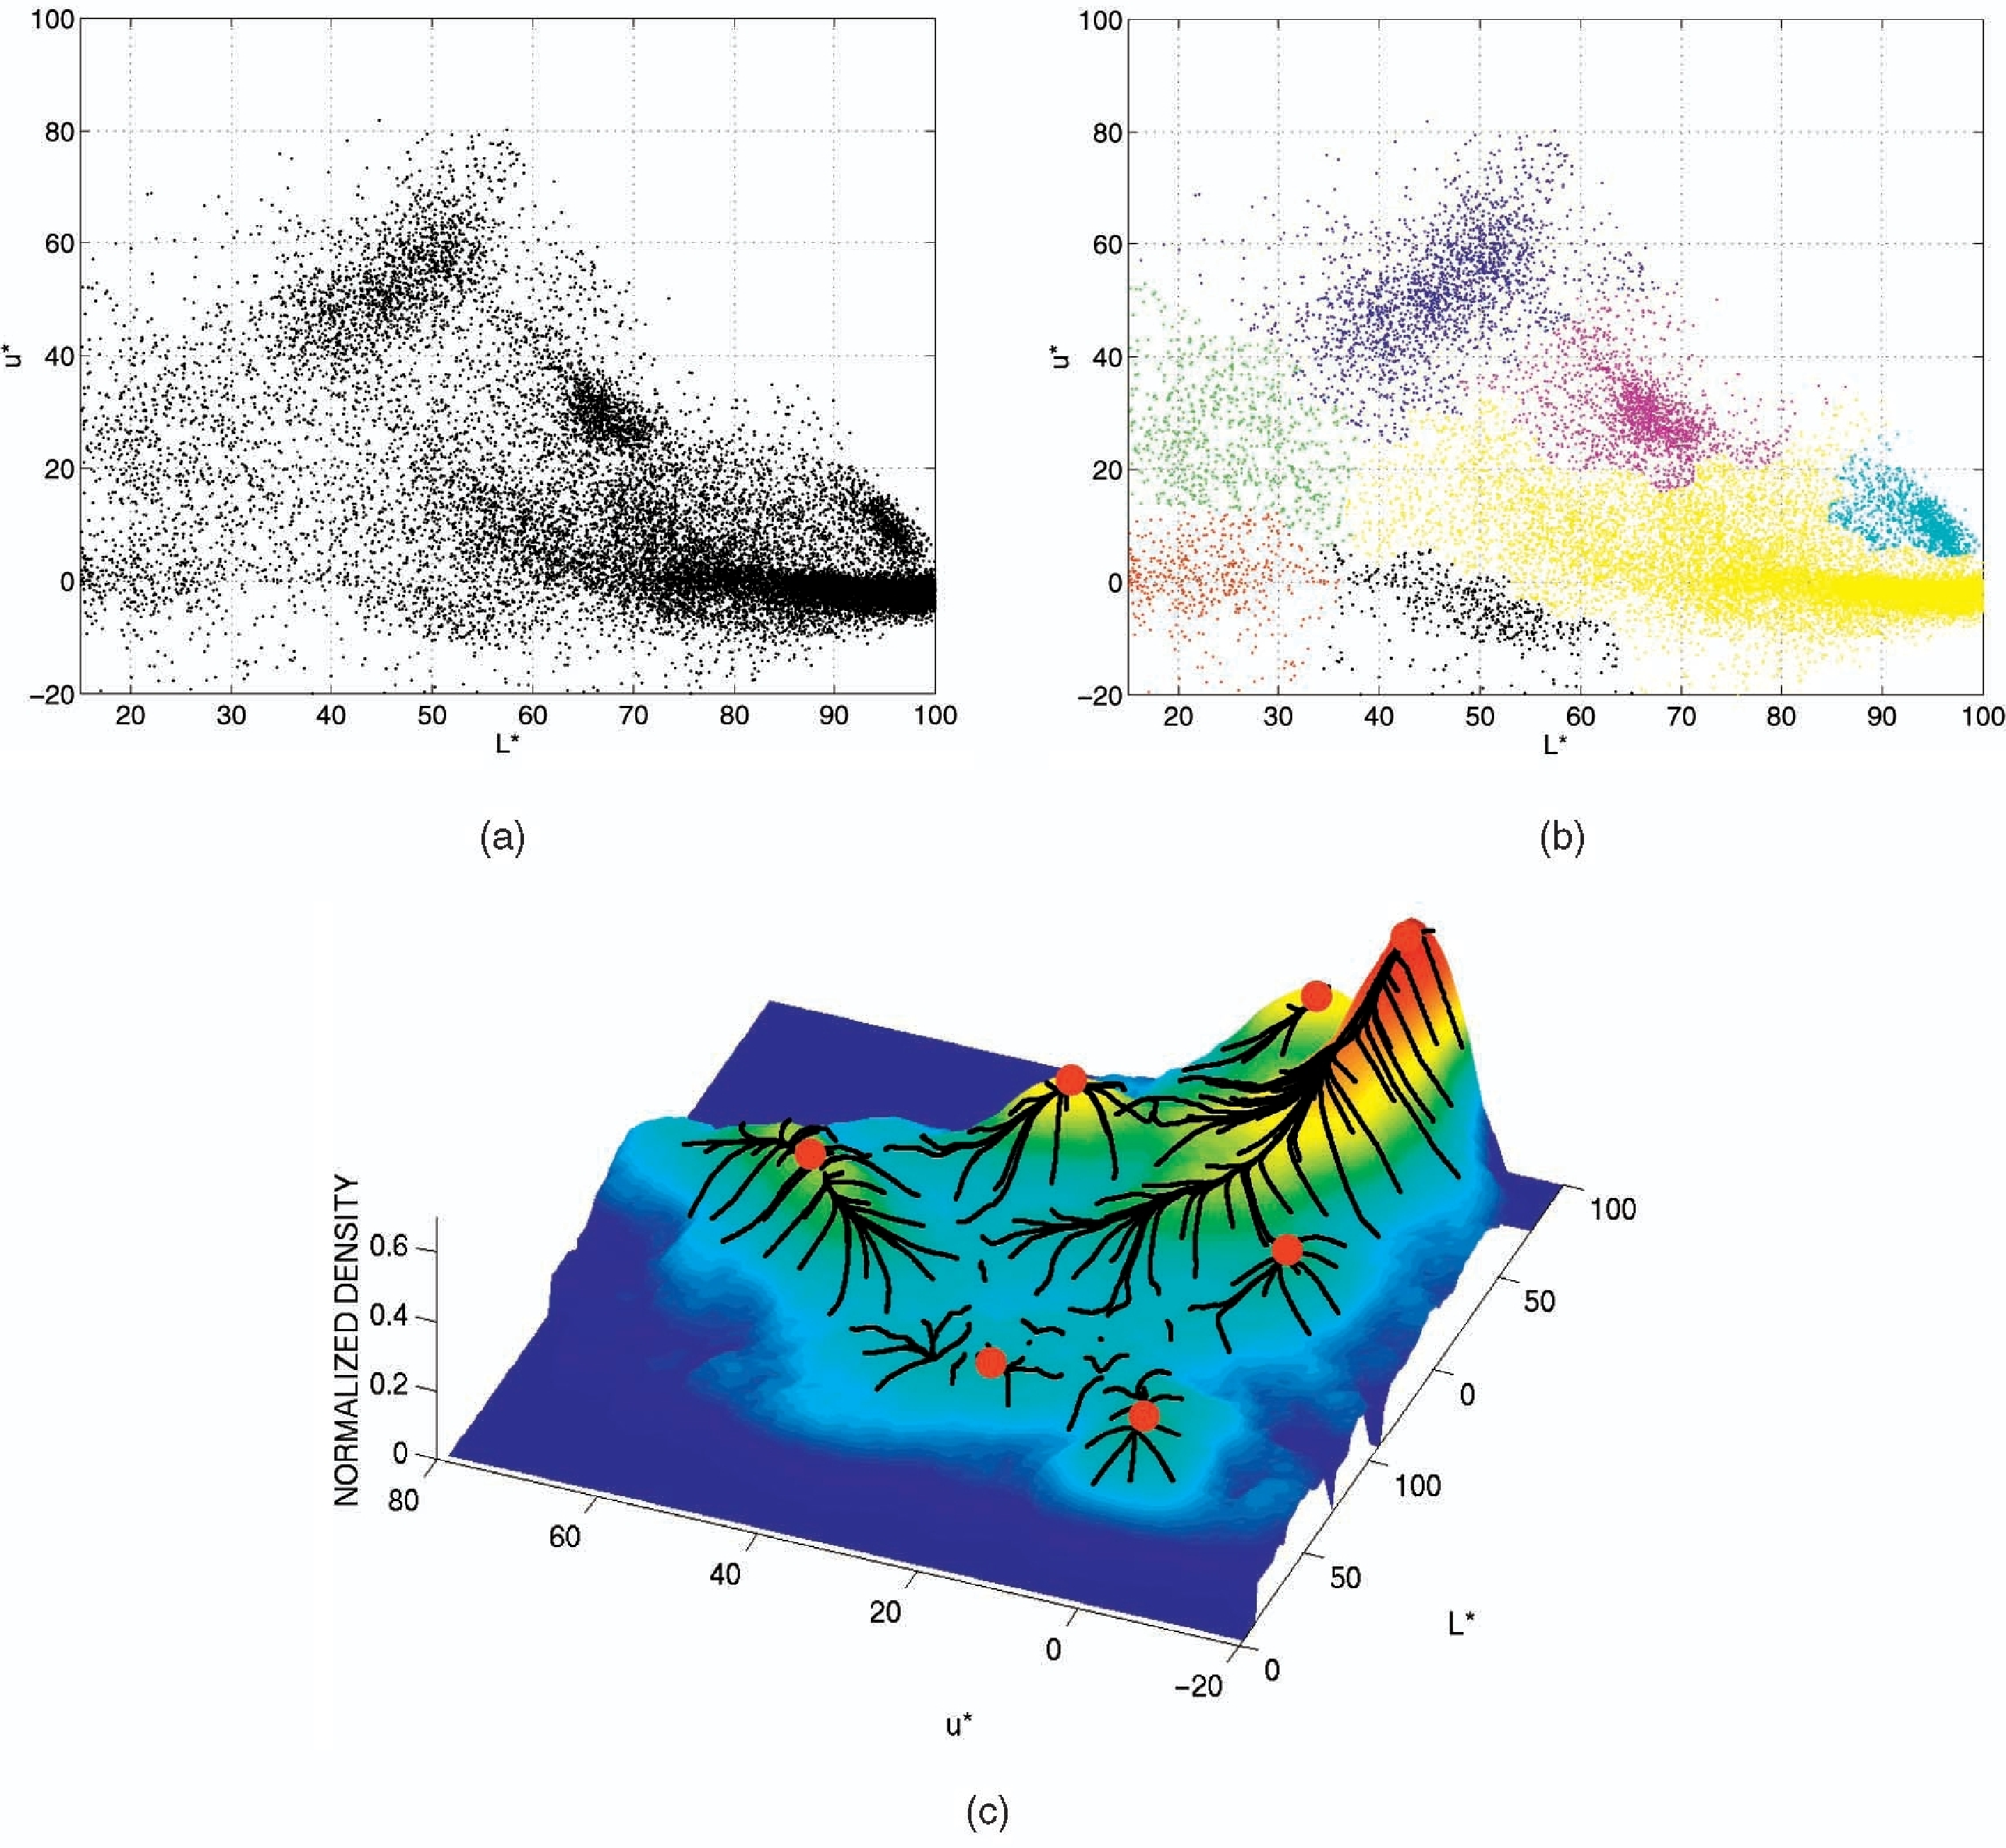
\includegraphics[height=0.65\textheight]{figs/PRML_meanShift2.pdf}
	\end{figure}
\end{frame}




%-------------------------------------------------------------
\subsubsection{\ \ \ \ 3. Boundary based methods}
%-------------------------------------------------------------
\begin{frame}
\frametitle{Boundary based methods}
\logoCSIPCPL\mypagenum
	\begin{block}{Definition:}A family of segmentation methods that rely on foreground object boundaries for segmentation.
	\end{block}
\end{frame}





\begin{frame}
\frametitle{Boundary based methods}
\logoCSIPCPL\mypagenum
	Boundary based methods are normally applied in two stages:
	\begin{enumerate}
		\item \textbf{Edge detection.}  Edge detection is accomplished by taking the first or second order derivative of the image.  This typically highlights the edges in the image.  Subsequent thresholding produces a binary image containing white edges on a black background, or vice
versa.
		\item \textbf{Boundary linking.}  The edges produced by the above method
are seldom completely connected.  Boundary linking is the process that tries to connect the edges.
	\end{enumerate}
\end{frame}





\begin{frame}
\frametitle{Boundary based methods}
\logoCSIPCPL\mypagenum
	\begin{itemize}
		\item Before discussing edge detection, note that point and line detection are implemented similarly to edge detection
		\item Therefore it is natural to start our discussion with point and line detection
	\end{itemize}
\end{frame}






%-------------------------------------------------------------
\subsubsection{\ \ \ \ \ \ \ \ Point detection}
%-------------------------------------------------------------
\begin{frame}
\frametitle{Boundary based methods}
\logoCSIPCPL\mypagenum
	Point detection mask:
	\begin{figure}[!htp]
		\includegraphics[width=2in]{figs/segmentation_MaskPointDetection.jpg}
	\end{figure}
\end{frame}






%-------------------------------------------------------------
\subsubsection{\ \ \ \ \ \ \ \ Line detection}
%-------------------------------------------------------------
\begin{frame}
\frametitle{Boundary based methods}
\logoCSIPCPL\mypagenum
	Line detection masks:
	\begin{figure}[!htp]
		\includegraphics[width=4.5in]{figs/segmentation_MaskLineDetection.jpg}
	\end{figure}
\end{frame}





\begin{frame}
\frametitle{Boundary based methods}
\logoCSIPCPL\mypagenum
	\begin{figure}[!htp]
	\subfigure[Input image]{
	    \includegraphics[width=1.5in]{figs/segmentation_MaskLineDetection_InputImage.jpg}}
	    \hspace{0.5cm}
	\subfigure[Output image]{
	    \includegraphics[width=1.5in]{figs/segmentation_MaskLineDetection_horizontal_OutputImage.jpg}}
	    \caption{Horizontal line detection}
	\end{figure}
\end{frame}






\begin{frame}
\frametitle{Boundary based methods}
\logoCSIPCPL\mypagenum
	\begin{figure}[!htp]
	\subfigure[Input image]{
	    \includegraphics[width=1.5in]{figs/segmentation_MaskLineDetection_InputImage.jpg}}
	    \hspace{0.5cm}
	\subfigure[Output image]{
	    \includegraphics[width=1.5in]{figs/segmentation_MaskLineDetection_vertical_OutputImage.jpg}}
	    \caption{Vertical line detection}
	\end{figure}
\end{frame}






\begin{frame}
\frametitle{Boundary based methods}
\logoCSIPCPL\mypagenum
	\begin{figure}[!htp]
	\subfigure[Input image]{
	    \includegraphics[width=1.5in]{figs/segmentation_MaskLineDetection_InputImage.jpg}}
	    \hspace{0.5cm}
	\subfigure[Output image]{
	    \includegraphics[width=1.5in]{figs/segmentation_MaskLineDetection_45p_OutputImage.jpg}}
	    \caption{$+45^o$ line detection}
	\end{figure}
\end{frame}



\begin{frame}
\frametitle{Boundary based methods}
\logoCSIPCPL\mypagenum
	\begin{figure}[!htp]
	\subfigure[Input image]{
	    \includegraphics[width=1.5in]{figs/segmentation_MaskLineDetection_InputImage.jpg}}
	    \hspace{0.5cm}
	\subfigure[Output image]{
	    \includegraphics[width=1.5in]{figs/segmentation_MaskLineDetection_45n_OutputImage.jpg}}
	    \caption{$-45^o$ line detection}
	\end{figure}
\end{frame}


%-------------------------------------------------------------
\subsubsection{\ \ \ \ \ \ \ \ Edge detection}
%-------------------------------------------------------------
\begin{frame}
\frametitle{Using first order derivatives}
\logoCSIPCPL\mypagenum
	\begin{block}{Definition:}
		A method to detect boundaries (edges) in an image using first order derivatives.
	\end{block}
\end{frame}




\begin{frame}
\frametitle{Using first order derivatives}
\logoCSIPCPL\mypagenum
	Continuous domain (2D) first order derivative:
	\begin{equation}
		\label{eqn:Cont2DFirstOrderDerivative}
		f'(x,y)=\|\nabla f\| = \sqrt{(\frac{\partial f}{\partial x})^2 + (\frac{\partial f}{\partial y})^2}
	\end{equation}
	This is also called the magnitude of the \emph{gradient}.
\end{frame}






\begin{frame}
\frametitle{Using first order derivatives}
\logoCSIPCPL\mypagenum
	A discrete approximation of the first order derivative is:	
	\begin{equation}
		f'[m,n] = f[m+1,n+1] - f[m,n]
		\label{eqn:Discrete2DFirstOrderDerivative}
	\end{equation}	
	This is called the \emph{Roberts} operator.  Other approximations
	are \emph{Prewitt} and \emph{Sobel}.
\end{frame}




\begin{frame}
\frametitle{Using first order derivatives}
\logoCSIPCPL\mypagenum
	\begin{figure}[!htp]
		\includegraphics[width=1.5in]{figs/segmentation_MaskFirstDerivative.jpg}
		\caption{First order derivative masks.  Top row: Roberts, middle row: Prewitt, bottom row: Sobel.} 
		\label{fig:MaskFirstDerivative}
	\end{figure}
\end{frame}




\begin{frame}
\frametitle{Using second order derivatives}
\logoCSIPCPL\mypagenum
	\begin{block}{Definition:}A method to detect boundaries (edges) in an image using second order derivatives.
	\end{block}
\end{frame}





\begin{frame}
\frametitle{Edge detection using second order derivatives}
\logoCSIPCPL\mypagenum
Continuous domain (2D) second order derivative:
\begin{equation}\label{eqn:Cont2DSecondOrderDerivative}
f''(x,y)=\nabla^2 f = (\frac{\partial^2 f}{\partial x^2}) +
(\frac{\partial^2 f}{\partial y^2})
\end{equation}
This is also called the \emph{laplacian}.
\end{frame}



\begin{frame}
\frametitle{using second order derivatives}
\logoCSIPCPL\mypagenum
	\begin{figure}[!htp]
		\includegraphics[width=2in]{figs/segmentation_MaskSecondDerivative(Laplacian).jpg}
		\caption{Two discrete approximations of the laplacian.}
		\label{fig:LaplacianMasks}
	\end{figure}
\end{frame}





\begin{frame}
\frametitle{Edge detection using second order derivatives}
\logoCSIPCPL\mypagenum
	\begin{figure}[!htp]
		\centering 
		\subfigure[Input image]
		{
		    \label{fig:sub:a}
		    \includegraphics[width=1in]{figs/segmentation_Mandril_gray_128x128.jpg}
		}
	    	\hspace{0.2cm}
		\subfigure[Output image]
		{
	    		\label{fig:sub:a}
	    		\includegraphics[width=1in]{figs/segmentation_MaskSecondDerivative(Laplacian)_OutputImage.jpg}
		}
		\caption{Application of laplacian.}
		\label{fig:ApplyingSecondOrderDerivatives}
	\end{figure}
\end{frame}





%-------------------------------------------------------------
\subsubsection{\ \ \ \ \ \ \ \ Boundary linking}
%-------------------------------------------------------------
\begin{frame}
\frametitle{Using exhaustive search}
\logoCSIPCPL\mypagenum
	\begin{block}{Definition:}
	A method to link broken edges in which boundaries are formed by finding every possible line between every possible pair of pixels, and picking those lines that 'seem' to work best.
	\end{block}
\end{frame}





\begin{frame}
\frametitle{Using least squares}
\logoCSIPCPL\mypagenum
	\begin{block}{Definition:}
		A method of fitting a piecewise linear or higher order spline curve through broken edges.
	\end{block}
	\begin{block}{Mathmatically:} 
		Given a set of points $(x_i, y_i)$, find the function $h(x)$ that minimizes the mean square error,
		\begin{equation}
			MSE = \frac{1}{N} \sum_{i=1}^{N} [y_i - h(x_i)]^2
		\end{equation}
	\end{block}
\end{frame}




\begin{frame}
\frametitle{Using Hough transform}
\logoCSIPCPL\mypagenum
	\begin{block}{Definition:}
		An efficient method to join broken edges that picks a line with the most votes in a discrete parameter space.
	\end{block}
\end{frame}



\begin{frame}
\frametitle{Using Hough transform}
\logoCSIPCPL\mypagenum
	\begin{itemize}
		\item Consider three points, $A(x_1, y_1)$, $B (x_2, y_2)$, and $C (x_3, y_3)$ lying on a straight line in cartesian space.
		\item Only one line passes through $A, B$ and $C$.  The equation of this line is $y=mx + c$
		\item The values of $m$ and $c$ that satisfy these three equations will give the desired line,
		\begin{align*}	
			y_1=m x_1 + c\\
			y_2=m x_2 + c\\
			y_3=m x_3 + c\\
			\label{eqn:3equations}
		\end{align*}
	\end{itemize}
\end{frame}





\begin{frame}
\frametitle{Using Hough transform}
\logoCSIPCPL\mypagenum
	\begin{itemize}
		\item The algebraic solution would be to solve all three equations simultaneously.
		\item The graphical solution would be to plot all three lines in the $(m,c)$ plane and find the point where all three lines intersect.
		\item The Hough transform presents an alternate computationally efficient procedure.
	\end{itemize}
\end{frame}




\begin{frame}
\framesubtitle{Using Hough transform}
\logoCSIPCPL\mypagenum
	\begin{itemize}
		\item We start by quantizing the parameter space, i.e., we divide the $(m,c)$ plane into a grid, called an \emph{Accumulator array}
		\item We use large grid cells to decrease computational complexity and accommodate slight variations in $(m,c)$ due to noise.
		\item For the point $A$, we use different values of $m$ in $y_1=m x_1 + c$ to get different values of $c$.
		\item For every pair $(m,c)$ so obtained, we increment the corresponding value in the $(m,c)$ grid.
		\item We repeat this procedure for $B$ and $C$.
		\item The grid cell that has the highest count in the end is the desired value of $(m,c)$.
	\end{itemize}
\end{frame}





\begin{frame}
\frametitle{Boundary linking using Hough transform}
\logoCSIPCPL\mypagenum
	\begin{itemize}
		\item A problem with using the slope intercept form of the equation of a line, $y=mx+c$, is that for a vertical line, the slope $m$ is infinite.
		\item This problem can be overcome by using the following parameterization,
		\begin{align*}
			x&=\rho cos(\theta)\\
			y&=\rho sin(\theta)
		\end{align*}
	\end{itemize}
\end{frame}






\begin{frame}
\frametitle{Boundary linking using Hough transform}
\logoCSIPCPL\mypagenum
	This yields the $normal$ form of a line,
	\begin{equation}
		\rho = x \ cos(\theta) + y \ sin(\theta)
	\end{equation}
	It is called the normal form because the desired line is normal to a line drawn from the origin to $(x,y)$.
\end{frame}




\begin{frame}
\frametitle{Boundary linking using Hough transform}
\logoCSIPCPL\mypagenum
	\begin{figure}[!htp]
		\includegraphics[width=2in]{figs/segmentation_NormalRepresentationOfLine.jpg}
		\caption{Normal representation of line.}
		\label{fig:NormalRepresentationOfLine}
	\end{figure}
\end{frame}






\begin{frame}
\frametitle{Boundary linking using Hough transform}
\logoCSIPCPL\mypagenum
	\begin{itemize}
		\item Therefore, to compute the Hough transform, use the $(\rho,
		\theta)$ space rather than the $(m,c)$ space
		\item This is explained next with an example
	\end{itemize}
\end{frame}







\begin{frame}
\frametitle{Boundary linking using Hough transform}
\logoCSIPCPL\mypagenum
	\begin{itemize}
		\item Consider three points on a line $(3,4)$, $(4,5)$ and $(5,6)$
		\item We need to find the line that goes through these points
		\item For the slope-intercept form, write the equation of each point as
			\begin{align*}
				4=3m+c \\
				5=4m+c \\
				6=5m+c
			\end{align*}
		\end{itemize}
\end{frame}






\begin{frame}
\frametitle{Boundary linking using Hough transform}
\logoCSIPCPL\mypagenum
	\begin{itemize}
		\item The algebraic solution is to solve these three equations to get $(m,c)=(1,1)$
		\item The graphical solution is to plot these three lines in the $(m,c)$ space and see that they intercept at $(m,c)=(1,1)$.
		\item The Hough transform solution is a discretized version of the graphical solution, and the cell $(m,c)=(1,1)$ gets the most number of votes
		\item The solution therefore is $y=x+1$
	\end{itemize}
\end{frame}





\begin{frame}
\frametitle{Boundary linking using Hough transform}
\logoCSIPCPL\mypagenum
	\begin{itemize}
		\item Now we solve this problem using the normal form
		\item For the normal form, write the equation of each point as
		\begin{align*}
			3cos(\theta)+4sin(\theta)=\rho \\
			4cos(\theta)+5sin(\theta)=\rho \\
			5cos(\theta)+6sin(\theta)=\rho
		\end{align*}
	\end{itemize}
\end{frame}







\begin{frame}
\frametitle{Boundary linking using Hough transform}
\logoCSIPCPL\mypagenum
	\begin{itemize}
		\item The algebraic solution is not straightforward.
		\item The graphical solution is to plot these three lines in the $(\rho, \theta)$ space and see that they intersect at $(\rho, \theta) = (-0.707, -\pi/4)$.
		\item The Hough transform solution is again a discretized version of the graphical solution and the cell $(\rho, \theta) = (-0.707, -\pi/4)$ gets the most number of votes.
		\item So a line with length $-0.707$ oriented at $\theta = -\pi/4$ is normal to our desired line. This line is $y=x+1$.
	\end{itemize}
\end{frame}







\begin{frame}
\frametitle{Boundary linking using Hough transform}
\logoCSIPCPL\mypagenum
	\begin{figure}[!htp]
		\includegraphics[width=2in]{figs/segmentation_HoughTransformSolution-Normal.jpg}
		\caption{Hough transform example.} \label{fig:HoughTransformExample}
	\end{figure}
\end{frame}






%===================================================
\subsection{\ \ \ \ 4. Watershed based methods}
%===================================================


\begin{frame}
\frametitle{Watershed based methods}
\logoCSIPCPL\mypagenum
	\begin{block}{Definition:}
	A family of segmentation methods that view an image as a topological surface described by three main features: \emph{regional minima}, \emph{catchment basins} and \emph{watershed lines}.  The image is segmented along the watershed lines.
	\end{block}
\end{frame}





\begin{frame}
\frametitle{Watershed based methods}
\logoCSIPCPL\mypagenum	
	\begin{figure}[!htp]
		\includegraphics[width=2in]{figs/segmentation_WatershedTopologicalFeatures.jpg}
		\caption{Topological features.}
		\label{fig:WatershedTopologicalFeatures}
	\end{figure}
\end{frame}





\begin{frame}
\frametitle{Watershed based methods}
\logoCSIPCPL\mypagenum
	\begin{itemize}
		\item If rain were to fall on such a topological surface, it would flow down the catchment basins and collect in the regional minima.
		\item The water level will rise and the catchment basins will fill up with water.
		\item At points where water coming from different basins would meet, dams are built.
		\item When the water level has reached the highest peak in the landscape, the process is stopped.
		\item As a result, the landscape is partitioned into basins (regions) separated by watershed lines (boundaries).
	\end{itemize}
\end{frame}





\begin{frame}
\frametitle{Immersion approach}
\logoCSIPCPL\mypagenum
	\begin{itemize}
		\item In the Immersion approach, we raise the water level not by raining down on the landscape, but by visualizing our landscape as
		being immersed in a lake with holes pierced in each of the regional minima.
		\item As the surface is slowly immersed into the lake, the water level will rise in each of the catchment basins, until a point will come when water from one basin will overflow into another.
		\item At this point, we build a dam on the ridge line separating the two basins.
		\item As this process continues, the entire image will be segmented using dams.
		\item These dams are the watershed lines.
	\end{itemize}
\end{frame}





\begin{frame}
\frametitle{Immersion approach}
\logoCSIPCPL\mypagenum
	We introduce three mathematical terms, and relate them to concepts of watershed segmentation:
	\begin{enumerate}
		\item Geodesic distance
		\item Geodesic Influence Zone
		\item Skeleton by Influence Zones (SKIZ)
	\end{enumerate}
\end{frame}





\begin{frame}
\frametitle{Immersion approach}
\logoCSIPCPL\mypagenum
	\begin{itemize}
		\item Two points $x$ and $y$ lie in region $f$.
		\item Several paths $P(x,y)$ can be drawn to join $x$ and $y$.
	\end{itemize}
	\begin{figure}[!htp]
		\includegraphics[width=2.5in]{figs/segmentation_WatershedGeodesicDistanceAndInfluenceZone.jpg}
	\end{figure}
\end{frame}





\begin{frame}
\frametitle{Immersion approach}
\logoCSIPCPL\mypagenum
	\begin{itemize}
		\item We pick the shortest path that completely lies in $f$.
		\item The length of this path is called the \emph{Geodesic Distance} $d_f(x,y)$,
	\end{itemize}
	\begin{equation}
		d_f(x,y)= min \{ length(P(x,y) \}
	\end{equation}
\end{frame}



\begin{frame}
\frametitle{Watershed based methods}
\logoCSIPCPL\mypagenum
	Region $f$ contains several connected components $m_i, i \in [1,k]$.  The union of these connected components is denoted by $M$,
	\begin{equation}
		M=\bigcup_{i \in [1,k]} m_i
	\end{equation}
	\begin{figure}[!htp]
		\includegraphics[width=2.5in]{figs/segmentation_WatershedGeodesicDistanceAndInfluenceZone.jpg}
	\end{figure}
\end{frame}





\begin{frame}
\frametitle{Immersion approach}
\logoCSIPCPL\mypagenum
	For every connected component $m_i$, we can create a buffer zone around it by taking the locus of points in $f$ whose geodesic distance to $m_i$ is less than the geodesic distance to any other connected component.	
	\begin{figure}[!htp]
		\includegraphics[width=2.5in]{figs/segmentation_WatershedGeodesicDistanceAndInfluenceZone.jpg}
	\end{figure}
\end{frame}






\begin{frame}
\frametitle{Immersion approach}
\logoCSIPCPL\mypagenum
	Such a buffer zone around connected component $m_i$ is called its \emph{Geodesic Influence Zone}, $c_f(m_i)$.  The union of all geodesic influence zones is denoted by $C_f$,
	\begin{align*}
		c_f(m_i)&=  \{ \ p \in f \ | \ d(p,m_i) < d(p,m_j), \ \ \ j \in [1,k], \ j \neq i \}\\
		C_f(M)&=\bigcup_{i \in [1,k]} c_f(m_i)
	\end{align*}
\end{frame}






\begin{frame}
\frametitle{Immersion approach}
\logoCSIPCPL\mypagenum
	The union of all connected components and geodesic influence zones is denoted by $X$,
	\begin{equation}
		X= M \cup C_f(M)
	\end{equation}
	\begin{figure}[!htp]	
		\includegraphics[width=2.5in]{figs/segmentation_WatershedGeodesicDistanceAndInfluenceZone.jpg}
	\end{figure}
\end{frame}





\begin{frame}
\frametitle{Immersion approach}
\logoCSIPCPL\mypagenum	
	Notice that the only points remaining in $f$ which do not belong to $X$ are the dividing lines between the geodesic influence zones.  These points are called the Skeleton by Influence Zones (SKIZ).
	\begin{equation}
	W_f = f/X
	\end{equation}
\end{frame}






\begin{frame}
\frametitle{Immersion approach}
\logoCSIPCPL\mypagenum
	We now relate these mathematical concepts to the topological
	representation of image $f$,	
	\begin{enumerate}
		\item \textbf{Regional minima.}  The regional minima in image $f$ are equivalent to connected components, $m_i$.
		\item \textbf{Catchment basins.}  The catchment basins in image $f$ are equivalent to the geodesic influence zones, $c_f(m_i)$.
		\item \textbf{Watershed basins.}  The watershed lines in image $f$ are equivalent to the skeleton by influence zones, $W_f$.
	\end{enumerate}
\end{frame}





\begin{frame}
\frametitle{Immersion approach}
\logoCSIPCPL\mypagenum
	When the water level is raised, we can have one of the following 3 situations, when looking from above:
	\begin{figure}[!htp]
		\includegraphics[width=4in]{figs/segmentation_WatershedInclusionRelations.jpg}
	\end{figure}
\end{frame}





\begin{frame}
\frametitle{Immersion approach}
\logoCSIPCPL\mypagenum
	In the left figure, all we see is water.
	\begin{figure}[!htp]
		\includegraphics[width=4in]{figs/segmentation_WatershedInclusionRelations.jpg}
	\end{figure}
\end{frame}





\begin{frame}
\frametitle{Immersion approach}
\logoCSIPCPL\mypagenum
	In the middle figure, the black portion is a minimum, and the blue water around it corresponds to its catchment basin (geodesic	influence zone).
	\begin{figure}[!htp]
		\includegraphics[width=4in]{figs/segmentation_WatershedInclusionRelations.jpg}
	\end{figure}
\end{frame}





\begin{frame}
\frametitle{Immersion approach}
\logoCSIPCPL\mypagenum
	In the right figure, we have two minima close to each other, andtheir catchment basins are close to each other.  We therefore need a skeleton by influenze zone (i.e. watershed line) to separate them.
	\begin{figure}[!htp]
		\includegraphics[width=4in]{figs/segmentation_WatershedInclusionRelations.jpg}
	\end{figure}
\end{frame}





\begin{frame}
\frametitle{Immersion approach}
\logoCSIPCPL\mypagenum
	In summary, the three situations discussed lead to the following
	segmentation:
	\begin{figure}[!htp]
		\includegraphics[width=4in]{figs/segmentation_WatershedRecursion.jpg}
	\end{figure}
\end{frame}

%####################################################################################################
\section{PRIOR WORK}
%####################################################################################################

%-------------------------------------
\subsection{\ \ \ \ 1992: Brown}
%-------------------------------------
\begin{frame}
\frametitle{Prior work: image registration survey}
\framesubtitle{}
\mypagenum
\myFootnoteCitation{1992_JNL_SURVEYreg_Brown}{Computing Surveys}
\end{frame}





%####################################################################################################
%####################################################################################################
%\bibliographystyle{ieee}
%\bibliography{c:/salman/work/writing/MyCitations}
\end{document}
%####################################################################################################

%####################################################################################################
